\documentclass[12pt,a4j]{jarticle}
%---------------------------------------------------
\usepackage[dvipdfmx]{graphicx}
\usepackage{amssymb}
\usepackage{amsmath}
\usepackage{ascmac}
\usepackage{setspace}
\usepackage{float}
\usepackage[dvipdfmx,usenames]{color}
\usepackage{colortbl}
\usepackage{algorithm}
\usepackage{algorithmic}
\usepackage{setspace}
\usepackage{udline}
%---------------------------------------------------
\makeatletter
\def\@maketitle{%
\begin{center}%
\let\footnote\thanks
\vspace*{80mm} % この量でタイトルの位置が下がる。
{\LARGE \@title \par}%
\vskip 1.5em%
{\large
\lineskip .5em%
\begin{tabular}[t]{c}%
\@author
\end{tabular}\par}%
\vskip 1em%
{\large \@date}%
\end{center}%
\par\vskip 1.5em}
\makeatother

\title{\Huge 教務支援システム\\内部設計書}
\date{\today}
\author{\large Outing Corporation}
\begin{document}

\maketitle

\newpage

\setcounter{tocdepth}{2}
\tableofcontents

\pagenumbering{arabic}
\newpage
% input
\section{動作環境}

\begin{itemize}

\item 動作環境\\
本システムの動作環境は以下の通りです.
\begin{itemize}
\item raspberry Pi 3 Model B
\item CPU:ARM Cortex-A53
\item GPU:Broadcom VideoCore IV
\item メモリ:LPDDR2 SDRAM 1 GB
\item ストレージ:4 GB eMMC / SDカードPIN
\item OS: Raspbian Stretch
\item webサーバ:Nginx 1.10.3
\item Appサーバ:Ruby on Rails 5.1.4
\item RDBMS:MySQL version 14.14
\end{itemize}

\item 使用ブラウザ
  \begin{itemize}
  \item Google Chrome version 62.0
  \item Firefox version 57.0
  \end{itemize}

\item 開発環境\\
本システムの開発環境は以下の通りです.
  \begin{itemize}
  \item OS:Windows10, ubuntu 16.04 LTS, MacOS Sierra, Raspbian Stretch
  \end{itemize}

\item 使用言語\\
本システムの開発環境は以下の通りです.
\begin{itemize}
\item Ruby on Rails version 5.1.4
\item ruby version 2.4.2
\item HTML5
\item CSS
\item JavaScript
\end{itemize}

\item サーバ:Raspberry Pi 3 Model B

\item データベース:MySQL version 14.14

\item webサーバ:Nginx 1.10.3

\item 文書作成ツール:LaTeX

\item バージョン管理:Git

\item 連絡ツール:Slack

\item 日程管理ツール:Google Calendar

\item UML図作成ツール:Power Point, Excel, A5:SQL Mk-2

\end{itemize}

\section{コード規約}
ファイル命名規則は原則Railsの命名規則に従う

\begin{itemize}
\item コード命名規則
  \begin{itemize}
  \item クラス名,モジュール名は原則UpperCamelCase
  \item 変数名,メソッド名は原則snake\_case
  \item 定数名は全て大文字で'\_'で区切る
\end{itemize}
\item コーディングスタイル
\begin{itemize}
  \item インデントには半角スペース 2 文字を使用する
  \item 文字コードはUTF-8とする
  \item 改行コードにはLFを使用する
  \end{itemize}
\end{itemize}

\newpage

\section{データベースの設計}
本システムで使用するデータベースMySQLのテーブルについて示します。また、ERモデルで表したER図式を図\ref{fig:ER}で示します。
\begin{figure}[h]
	\begin{center}
	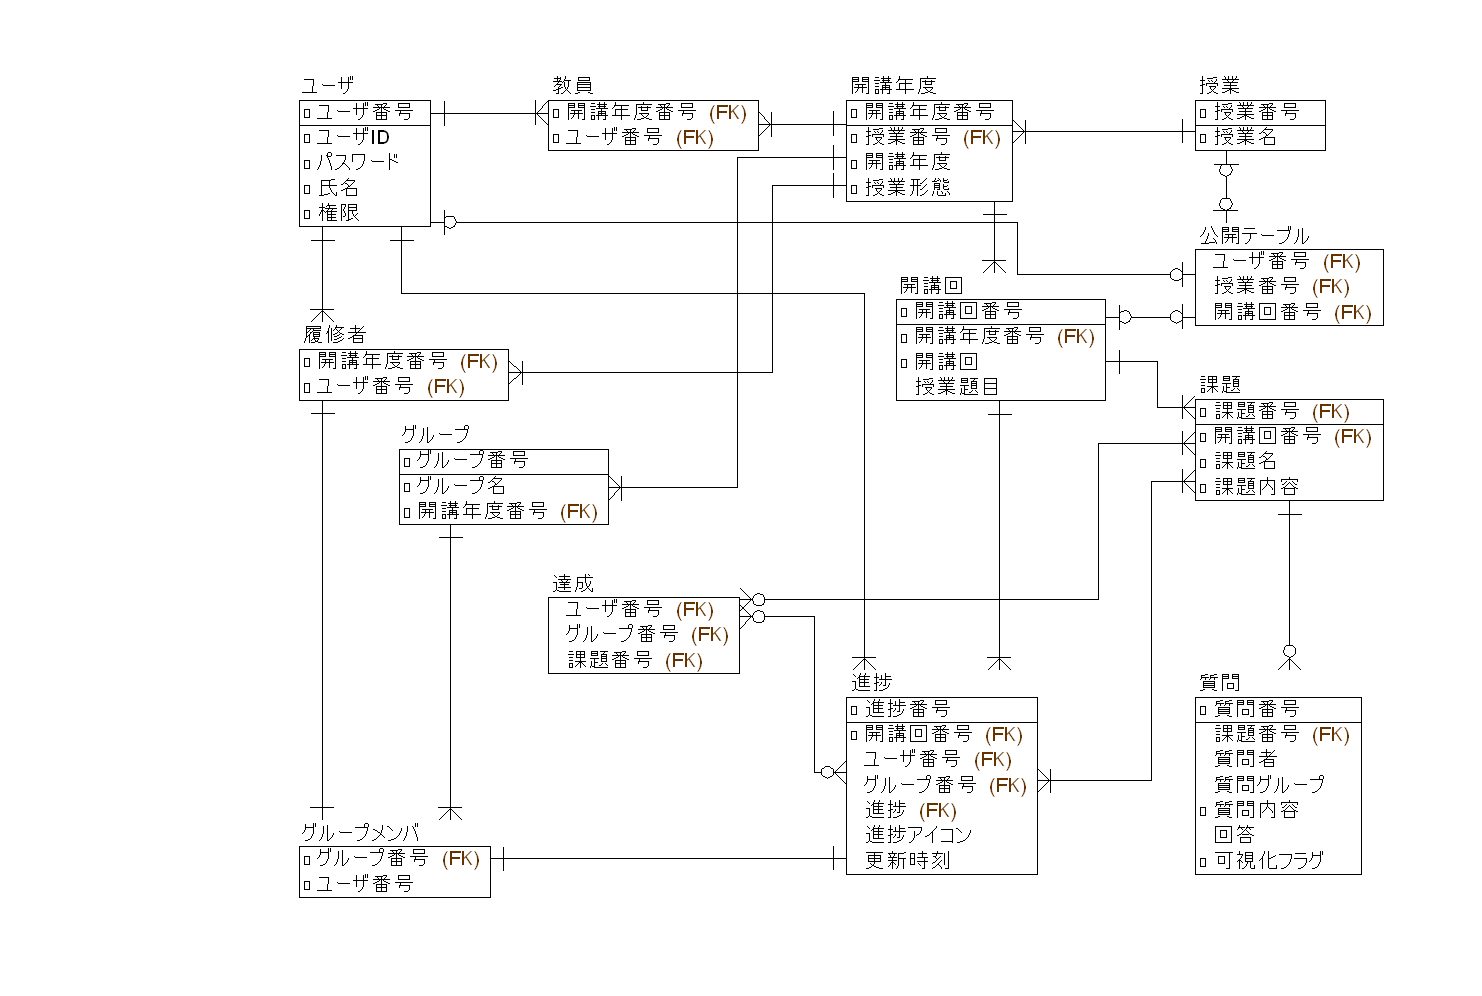
\includegraphics[width=1\linewidth,clip]{./img/er.png}
	\caption{実体関連図式}
	\label{fig:ER}
	\end{center}
\end{figure}

\newpage
\subsection{ユーザテーブル}
本システム利用者のユーザ情報を格納します。権限が「学生」であるユーザ情報は、登録日から設定した年が経過すると削除されます。各フィールドの概要は以下の通りです。また、ユーザテーブルの詳細は表\ref{ユーザテーブル}で示します。
\begin{itemize}
	\item ユーザ番号(USER\_NO):\\ユーザテーブルの主キー
	\item ユーザID(USER\_ID):\\システムにおいてユーザを一意に定める名前
	\item パスワード(PASSWORD):\\ユーザの識別・確認に用いるパスワード
	\item 氏名(USER\_NAME):\\ユーザ本人の名前
	\item 権限(AUTHORITY):\\ユーザに「教員」、「アシスタント」または「学生」のいずれかの権限を与える
\end{itemize}

	\begin{table}[h]
		\centering
		\caption{ユーザテーブル(TB\_USER)}
		\label{ユーザテーブル}
		\begin{tabular}{|l|l|l|c|l|}
		\hline
		フィールド & 型  & 外部キー & Null & オプション\\ \hline\hline
		\ul{ユーザ番号} & \begin{tabular}[c]{@{}l@{}}INT\\ UNSIGNED\end{tabular} &  & No & AUTO\_INCREMENT\\ \hline
		ユーザID & VARCHAR(32) & & No & UNIQUE\\ \hline
		パスワード & VARCHAR(64) & & No & \\ \hline
		氏名 & VARCHAR(16) &  & No  &\\ \hline
		権限 & ENUM & & No & \\ \hline
		\end{tabular}
	\end{table}

\newpage

\subsection{履修者テーブル}
受講するユーザ情報を格納します。各フィールドの概要は以下の通りです。また、履修者テーブルの詳細は表\ref{履修者テーブル}で示します。
\begin{itemize}
	\item 開講年度番号(LECTURE\_YEAR\_NO):\\何年度の何の授業であるかを示す
	\item ユーザ番号(USER\_NO):\\授業を履修する学生ユーザ
\end{itemize}

	\begin{table}[h]
		\centering
		\caption{履修者テーブル(TB\_STUDENT)}
		\label{履修者テーブル}
		\begin{tabular}{|l|l|l|c|l|}
		\hline
		フィールド & 型 & 外部キー & Null & オプション \\ \hline\hline
		開講年度番号 & \begin{tabular}[c]{@{}l@{}}INT\\ UNSIGNED\end{tabular} & 開講年度 & No & \\ \hline
		ユーザ番号 & \begin{tabular}[c]{@{}l@{}}INT\\ UNSIGNED\end{tabular} & ユーザ & No & \\ \hline
		\end{tabular}
	\end{table}

\subsection{グループテーブル}
授業のために作成されたグループ情報を格納します。各フィールドの概要は以下の通りです。また、グループテーブルの詳細は表\ref{グループテーブル}で示します。
\begin{itemize}
	\item グループ番号(GROUP\_NO):\\グループテーブルの主キー
	\item グループ名(GROUP\_NAME):\\グループの名前
	\item 開講年度番号(LECTURE\_YEAR\_NO):\\何年度の何の授業のために作成されたかを示す
\end{itemize}

	\begin{table}[h]
		\centering
		\caption{グループテーブル(TB\_GROUP)}
		\label{グループテーブル}
		\begin{tabular}{|l|l|l|c|l|}
		\hline
		フィールド & 型 & 外部キー & Null & オプション\\ \hline\hline
		\ul{グループ番号} & \begin{tabular}[c]{@{}l@{}}INT\\ UNSIGNED\end{tabular} & & No & AUTO\_INCREMENT \\ \hline
		グループ名 & VARCHAR(16) & & No & \\ \hline
		開講年度番号 & \begin{tabular}[c]{@{}l@{}}INT\\ UNSIGNED\end{tabular} & 授業 & No & \\ \hline
		\end{tabular}
	\end{table}

\subsection{グループメンバテーブル}
授業のために作成されたグループに所属しているユーザ情報を格納します。各フィールドの概要は以下の通りです。また、グループメンバテーブルの詳細は表\ref{グループメンバテーブル}で示します。
\begin{itemize}
	\item グループ番号(GROUP\_NO):\\何年度の何の授業のために作成されたグループであるかを示す
	\item ユーザ番号(USER\_NO):\\グループに所属している学生
\end{itemize}

	\begin{table}[h]
		\centering
		\caption{グループメンバテーブル(TB\_GROUP\_MEMBER)}
		\label{グループメンバテーブル}
		\begin{tabular}{|l|l|l|c|l|}
		\hline
		フィールド & 型 & 外部キー & Null & オプション\\ \hline\hline
		グループ番号 & \begin{tabular}[c]{@{}l@{}}INT\\ UNSIGNED\end{tabular} & グループ & No & \\ \hline
		ユーザ番号 & \begin{tabular}[c]{@{}l@{}}INT\\ UNSIGNED\end{tabular} & ユーザ & No & \\ \hline
		\end{tabular}
	\end{table}
\subsection{授業テーブル}
本システムを利用する授業の情報を格納します。各フィールドの概要は以下の通りです。また、授業テーブルの詳細は表\ref{授業テーブル}で示します。
\begin{itemize}
	\item 授業番号(LECTURE\_NO):\\授業テーブルの主キー
	\item 授業名(LECTURE\_NAME):\\授業の名前
\end{itemize}

	\begin{table}[h]
		\centering
		\caption{授業テーブル(TB\_LECTURE)}
		\label{授業テーブル}
		\begin{tabular}{|l|l|l|c|l|}
		\hline
		フィールド & 型 & 外部キー & Null & オプション \\ \hline\hline
		\ul{授業番号} & \begin{tabular}[c]{@{}l@{}}INT\\ UNSIGNED\end{tabular} & & No & AUTO\_INCREMENT \\ \hline
		授業名 & VARCHAR(32) & & No & UNIQUE \\ \hline
		\end{tabular}
	\end{table}
\subsection{開講年度テーブル}
開講された年度を含めた授業情報を格納します。各フィールドの概要は以下の通りです。また、開講年度テーブルの詳細は表\ref{開講年度テーブル}で示します。
\begin{itemize}
	\item 開講年度番号(LECTURE\_YEAR\_NO):\\開講年度テーブルの主キー
	\item 授業番号(LECTURE\_NO):\\授業を示す
	\item 開講年度(LECTURE\_YEAR):\\開講された年度を示す
	\item 授業形態(LECTURE\_STYLE):\\授業の進捗を「個人」または「グループ」のどちらで表示するかを示す
\end{itemize}

	\begin{table}[h]
		\centering
		\caption{開講年度テーブル(TB\_LECTURE\_YEAR)}
		\label{開講年度テーブル}
		\begin{tabular}{|l|l|l|c|l|}
		\hline
		フィールド & 型 & 外部キー & Null & オプション \\ \hline\hline
		\ul{開講年度番号} & \begin{tabular}[c]{@{}l@{}}INT\\ UNSIGNED\end{tabular} & & No & AUTO\_INCREMENT \\ \hline
		授業番号 & \begin{tabular}[c]{@{}l@{}}INT\\ UNSIGNED\end{tabular} & 授業 & No & \\ \hline
		開講年度 & \begin{tabular}[c]{@{}l@{}}SMALLINT\\ UNSIGNED\end{tabular} & & No & \\ \hline
		授業形態 & ENUM & & No & \\ \hline
		\end{tabular}
	\end{table}

\subsection{開講回テーブル}
回ごとの授業情報を格納します。各フィールドの概要は以下の通りです。また、開講回テーブルの詳細は表\ref{開講回テーブル}で示します。
\begin{itemize}
	\item 開講回番号(LECTURE\_TIMES\_NO):\\開講回テーブルの主キー
	\item 開講年度番号(LECTURE\_YEAR\_NO):\\何年度の何の授業であるかを示す
	\item 開講回(LECTURE\_TIMES):\\何年度の何の授業の何回目に開講されたかを示す
	\item 授業題目(LECTURE\_TITLE):\\開講された回ごとの授業概要を示す
\end{itemize}

	\begin{table}[h]
		\centering
		\caption{開講回テーブル(TB\_LECTURE\_TIMES)}
		\label{開講回テーブル}
		\begin{tabular}{|l|l|l|c|l|}
		\hline
		フィールド & 型 & 外部キー & Null & オプション \\ \hline\hline
		\ul{開講回番号} & \begin{tabular}[c]{@{}l@{}}INT\\ UNSIGNED\end{tabular} &  & No & AUTO\_INCREMENT \\ \hline
		開講年度番号 & \begin{tabular}[c]{@{}l@{}}INT\\ UNSIGNED\end{tabular} & 開講年度 & No & \\ \hline
		開講回 & \begin{tabular}[c]{@{}l@{}}TINYINT\\ UNSIGNED\end{tabular} & & No & \\ \hline
		授業題目 & VARCHAR(256) & & & \\ \hline
		\end{tabular}
	\end{table}
\subsection{公開テーブル}
現在開講されている授業情報を格納します。各フィールドの概要は以下の通りです。また、公開テーブルの詳細は表\ref{公開テーブル}で示します。
\begin{itemize}
	\item ユーザ番号(USER\_NO):\\講義を開講した管理者を示す
	\item 授業番号(LECTURE\_NO):\\開講されている授業を示す
	\item 開講回番号(LECTURE\_TIMES\_NO):\\開講されている回を示す
\end{itemize}

	\begin{table}[h]
		\centering
		\caption{公開テーブル(TB\_OPEN\_LECTURE)}
		\label{公開テーブル}
		\begin{tabular}{|l|l|l|c|l|}
		\hline
		フィールド & 型 & 外部キー & Null & オプション \\ \hline\hline
		ユーザ番号 & \begin{tabular}[c]{@{}l@{}}INT\\ UNSIGNED\end{tabular} & ユーザ  & & \\ \hline
		授業番号 & \begin{tabular}[c]{@{}l@{}}INT\\ UNSIGNED\end{tabular} & 授業 &  & \\ \hline
		開講回番号 & \begin{tabular}[c]{@{}l@{}}INT\\ UNSIGNED\end{tabular} & 開講回 & No & \\ \hline
		\end{tabular}
	\end{table}

\subsection{課題テーブル}
授業の回ごとに提示する課題情報を格納します。各フィールドの概要は以下の通りです。また、課題テーブルの詳細は表\ref{課題テーブル}で示します。
\begin{itemize}
	\item 課題番号(PROBLEM\_NO):\\課題テーブルの主キー
	\item 開講回番号(LECTURE\_TIMES\_NO):\\何年度の何の授業の何回目の授業であるかを示す
	\item 課題名(PROBLEM\_NAME):\\授業回ごとに提示される課題の番号
	\item 課題内容(PROBLEM\_CONTENT):\\授業回ごとに提示される課題の内容
\end{itemize}

	\begin{table}[h]
		\centering
		\caption{課題テーブル(TB\_PROBLEM)}
		\label{課題テーブル}
		\begin{tabular}{|l|l|l|c|l|}
		\hline
		フィールド & 型 & 外部キー & Null & オプション \\ \hline\hline
		\ul{課題番号} & \begin{tabular}[c]{@{}l@{}}INT\\ UNSIGNED\end{tabular} & & No & AUTO\_INCREMENT \\ \hline
		開講回番号 & \begin{tabular}[c]{@{}l@{}}INT\\ UNSIGNED\end{tabular} & 開講回 & No & \\ \hline
		課題名 & VARCHAR(8) & & No  & \\ \hline
		課題内容 & VARCHAR(512) & & No & \\ \hline
		\end{tabular}
	\end{table}
\subsection{進捗テーブル}
授業回ごとの学生の課題の進捗情報を格納します。進捗情報は授業時間内のみで使用するため、授業終了から一定期間後に格納された情報は削除されます。各フィールドの概要は以下の通りです。また、進捗テーブルの詳細は表\ref{進捗テーブル}で示します。
\begin{itemize}
	\item 進捗番号(PROGRESS_NO):\\進捗テーブルの主キー
	\item 開講回番号(LECTURE\_TIMES\_NO):\\何年度の何の授業の何回目の授業であるかを示す
	\item ユーザ番号(USER\_NO):\\進捗を確認する対象である受講者
	\item グループ番号(GROUP\_NO):\\進捗を確認する対象である受講グループ
	\item 進捗アイコン(PROGRESS\_ICON):\\進捗確認画面で表示されるアイコンの種類
	\item 更新時刻(UPDATE\_TIME):\\進捗の最終更新時刻
\end{itemize}

	\begin{table}[h]
		\centering
		\caption{進捗テーブル(TB\_PROGRESS)}
		\label{進捗テーブル}
		\begin{tabular}{|l|l|l|c|l|}
		\hline
		フィールド & 型 & 外部キー & Null & オプション \\ \hline\hline
		\ul{進捗番号} & \begin{tabular}[c]{@{}l@{}}INT\\ UNSIGNED\end{tabular} & & No & AUTO\_INCREMENT \\ \hline
		開講回番号 & \begin{tabular}[c]{@{}l@{}}INT\\ UNSIGNED\end{tabular} & 開講回 & No & \\ \hline
		ユーザ番号 & \begin{tabular}[c]{@{}l@{}}INT\\ UNSIGNED\end{tabular} & ユーザ  & & \\ \hline
		グループ番号 & \begin{tabular}[c]{@{}l@{}}INT\\ UNSIGNED\end{tabular} & グループ & & \\ \hline
		進捗アイコン & ENUM & & & \\ \hline
		更新時刻 & TIME & & & \\ \hline
		\end{tabular}
	\end{table}

\newpage

\subsection{質問テーブル}
授業回ごとに出た質問の情報を格納します。各フィールドの概要は以下の通りです。また、質問テーブルの詳細は表\ref{質問テーブル}で示します。
\begin{itemize}
	\item 質問番号(PROBLEM\_NO):\\質問テーブルの主キー
	\item 質問者(USER\_NAME):\\質問をした学生
	\item 質問グループ(GROUP\_NAME):\\質問をしたグループ
	\item 質問内容(QUESTION\_CONTENT):\\課題に対する質問の内容
	\item 回答(REPLY):\\質問に対する回答
	\item 可視化フラグ(VISIBLE\_FLAG):\\過去に出た質問の中で、学生に質問や回答を表示させるかどうかのフラグ
\end{itemize}

	\begin{table}[h]
		\centering
		\caption{質問テーブル(TB\_QUESTION)}
		\label{質問テーブル}
		\begin{tabular}{|l|l|l|c|l|}
		\hline
		フィールド & 型 & 外部キー & Null & オプション \\ \hline\hline
		\ul{質問番号}QUESTION\_NO & \begin{tabular}[c]{@{}l@{}}INT\\ UNSIGNED\end{tabular} & & No & AUTO\_INCREMENT \\ \hline
		課題番号 & \begin{tabular}[c]{@{}l@{}}INT\\ UNSIGNED\end{tabular} & 課題 &  & \\ \hline
		質問者 & VARCHAR(16) & & & \\ \hline
		質問グループ & VARCHAR(16) & & & \\ \hline
		質問内容 & VARCHAR(512) & & No & \\ \hline
		回答 & VARCHAR(512) & & & \\ \hline
		可視化フラグ & BOOLEAN &  & No & DEFAULT TRUE\\ \hline
		\end{tabular}
	\end{table}

\subsection{達成テーブル}
履修者が達成した課題情報を格納します。各フィールドの概要は以下の通りです。また、達成テーブルの詳細は表\ref{達成テーブル}で示します。
\begin{itemize}
	\item ユーザ番号(USER\_NO):\\進捗確認の対象である学生
	\item グループ番号(GROUP\_NO):\\進捗確認の対象であるグループ
	\item 課題番号(PROBLEM\_NO):\\達成した課題
\end{itemize}

	\begin{table}[h]
		\centering
		\caption{達成テーブル(TB\_ACHIEVMENT)}
		\label{達成テーブル}
		\begin{tabular}{|l|l|l|c|l|}
		\hline
		フィールド & 型 & 外部キー & Null & オプション\\ \hline\hline
		ユーザ番号 & \begin{tabular}[c]{@{}l@{}}INT\\ UNSIGNED\end{tabular} & 進捗  & & \\ \hline
		グループ番号 & \begin{tabular}[c]{@{}l@{}}INT\\ UNSIGNED\end{tabular} & 進捗 & & \\ \hline
		課題番号 & \begin{tabular}[c]{@{}l@{}}INT\\ UNSIGNED\end{tabular} & 課題 & & \\ \hline
		\end{tabular}
	\end{table}

\newpage
\section{各サブシステムのフローチャート}
各サブシステムのフローチャートを示します。

\subsection{質問閲覧サブシステム}

\begin{figure}[htbp]
  \begin{center}
    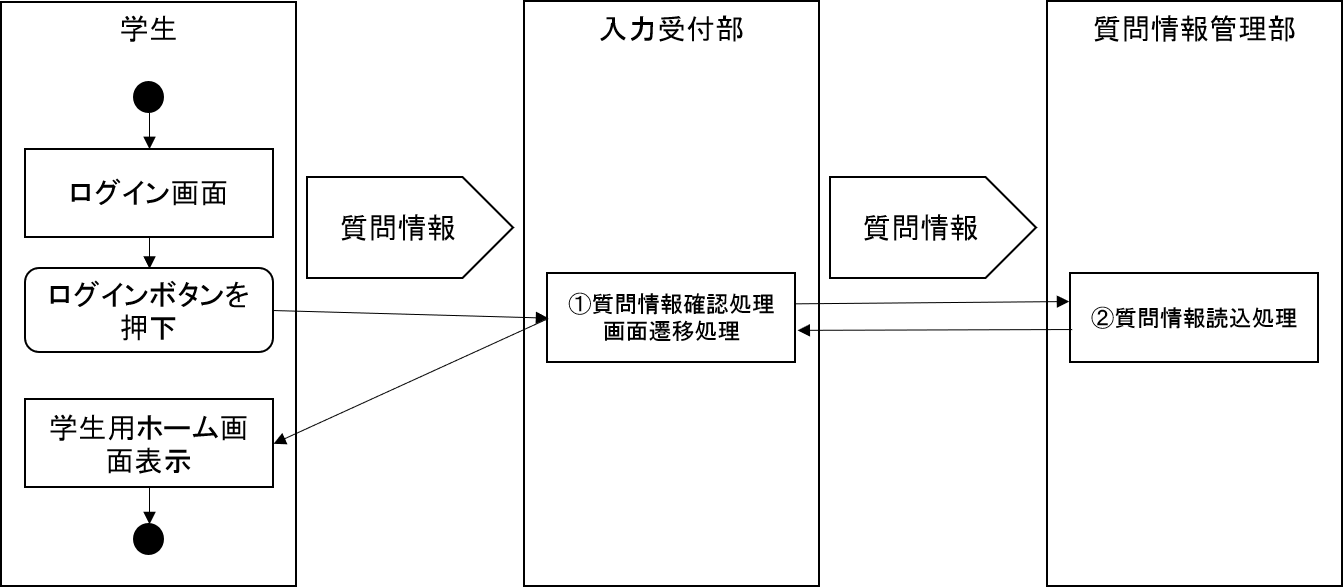
\includegraphics[width=1\linewidth,clip]{./img/質問閲覧システム}
    \caption{質問閲覧システムのフローチャート}\label{fig:03}
  \end{center}
\end{figure}

\newpage
\section{ルーティングとMVC}
\subsection{ルーティング}
Railsの規約に従ったurl規則を以下の表に定義します。
呼び出されたurlとHTTPメソッドによってRailsで呼び出すcontrollerのアクションを定義します。

\begin{table}[]
\centering
\caption{ルーティング一覧}
\label{my-label}
\begin{tabular}{lllll}
\cline{1-4}
\multicolumn{1}{|l|}{No.} & \multicolumn{1}{l|}{url}                 & \multicolumn{1}{l|}{METHOD} & \multicolumn{1}{l|}{Controller\#Action}       &  \\ \cline{1-4}
\multicolumn{1}{|l|}{---} & \multicolumn{1}{l|}{---}                 & \multicolumn{1}{l|}{----}   & \multicolumn{1}{l|}{----------}               &  \\ \cline{1-4}
\multicolumn{1}{|l|}{1}   & \multicolumn{1}{l|}{/login}              & \multicolumn{1}{l|}{GET}    & \multicolumn{1}{l|}{sessions\#new}            &  \\ \cline{1-4}
\multicolumn{1}{|l|}{2}   & \multicolumn{1}{l|}{}                    & \multicolumn{1}{l|}{POST}   & \multicolumn{1}{l|}{sessions\#create}         &  \\ \cline{1-4}
\multicolumn{1}{|l|}{3}   & \multicolumn{1}{l|}{/logout}             & \multicolumn{1}{l|}{DELETE} & \multicolumn{1}{l|}{sessions\#destroy}        &  \\ \cline{1-4}
\multicolumn{1}{|l|}{4}   & \multicolumn{1}{l|}{/not\_open}          & \multicolumn{1}{l|}{GET}    & \multicolumn{1}{l|}{static\_pages\#not\_open} &  \\ \cline{1-4}
\multicolumn{1}{|l|}{5}   & \multicolumn{1}{l|}{/home}               & \multicolumn{1}{l|}{GET}    & \multicolumn{1}{l|}{static\_pages\#home}      &  \\ \cline{1-4}
\multicolumn{1}{|l|}{6}   & \multicolumn{1}{l|}{/admin}              & \multicolumn{1}{l|}{GET}    & \multicolumn{1}{l|}{static\_pages\#admin}     &  \\ \cline{1-4}
\multicolumn{1}{|l|}{7}   & \multicolumn{1}{l|}{/signup}             & \multicolumn{1}{l|}{GET}    & \multicolumn{1}{l|}{users\#new}               &  \\ \cline{1-4}
\multicolumn{1}{|l|}{8}   & \multicolumn{1}{l|}{/users}              & \multicolumn{1}{l|}{POST}   & \multicolumn{1}{l|}{users\#create}            &  \\ \cline{1-4}
\multicolumn{1}{|l|}{9}   & \multicolumn{1}{l|}{/users/:id}          & \multicolumn{1}{l|}{PATCH}  & \multicolumn{1}{l|}{users\#update}            &  \\ \cline{1-4}
\multicolumn{1}{|l|}{10}  & \multicolumn{1}{l|}{/users/:id/edit}     & \multicolumn{1}{l|}{GET}    & \multicolumn{1}{l|}{users\#edit}              &  \\ \cline{1-4}
\multicolumn{1}{|l|}{11}  & \multicolumn{1}{l|}{/students}           & \multicolumn{1}{l|}{POST}   & \multicolumn{1}{l|}{students\#create}         &  \\ \cline{1-4}
\multicolumn{1}{|l|}{12}  & \multicolumn{1}{l|}{/students/new}       & \multicolumn{1}{l|}{GET}    & \multicolumn{1}{l|}{students\#new}            &  \\ \cline{1-4}
\multicolumn{1}{|l|}{13}  & \multicolumn{1}{l|}{/questions}          & \multicolumn{1}{l|}{GET}    & \multicolumn{1}{l|}{questions\#index}         &  \\ \cline{1-4}
\multicolumn{1}{|l|}{14}  & \multicolumn{1}{l|}{}                    & \multicolumn{1}{l|}{POST}   & \multicolumn{1}{l|}{questions\#create}        &  \\ \cline{1-4}
\multicolumn{1}{|l|}{15}  & \multicolumn{1}{l|}{/questions/new}      & \multicolumn{1}{l|}{GET}    & \multicolumn{1}{l|}{questions\#new}           &  \\ \cline{1-4}
\multicolumn{1}{|l|}{16}  & \multicolumn{1}{l|}{/questions/:id}      & \multicolumn{1}{l|}{DELETE} & \multicolumn{1}{l|}{questions\#delete}        &  \\ \cline{1-4}
\multicolumn{1}{|l|}{17}  & \multicolumn{1}{l|}{/progress}           & \multicolumn{1}{l|}{GET}    & \multicolumn{1}{l|}{progress\#index}          &  \\ \cline{1-4}
\multicolumn{1}{|l|}{18}  & \multicolumn{1}{l|}{/progress/:id}       & \multicolumn{1}{l|}{PATCH}  & \multicolumn{1}{l|}{progress\#update}         &  \\ \cline{1-4}
\multicolumn{1}{|l|}{19}  & \multicolumn{1}{l|}{/achievements}       & \multicolumn{1}{l|}{POST}   & \multicolumn{1}{l|}{achievements\#create}     &  \\ \cline{1-4}
\multicolumn{1}{|l|}{20}  & \multicolumn{1}{l|}{/lectures}           & \multicolumn{1}{l|}{POST}   & \multicolumn{1}{l|}{lectures\#create}         &  \\ \cline{1-4}
\multicolumn{1}{|l|}{21}  & \multicolumn{1}{l|}{/lectures/new}       & \multicolumn{1}{l|}{GET}    & \multicolumn{1}{l|}{lectures\#new}            &  \\ \cline{1-4}
\multicolumn{1}{|l|}{22}  & \multicolumn{1}{l|}{/years}              & \multicolumn{1}{l|}{GET}    & \multicolumn{1}{l|}{years\#index}             &  \\ \cline{1-4}
\multicolumn{1}{|l|}{23}  & \multicolumn{1}{l|}{/lecture\_times}     & \multicolumn{1}{l|}{GET}    & \multicolumn{1}{l|}{lecture\_times\#index}    &  \\ \cline{1-4}
\multicolumn{1}{|l|}{24}  & \multicolumn{1}{l|}{/lecture\_times/new} & \multicolumn{1}{l|}{GET}    & \multicolumn{1}{l|}{lecture\_times\#new}      &  \\ \cline{1-4}
\multicolumn{1}{|l|}{25}  & \multicolumn{1}{l|}{/questions}          & \multicolumn{1}{l|}{GET}    & \multicolumn{1}{l|}{questions\#index}         &  \\ \cline{1-4}
\multicolumn{1}{|l|}{26}  & \multicolumn{1}{l|}{/problem}            & \multicolumn{1}{l|}{PATCH}  & \multicolumn{1}{l|}{problems\#update}         &  \\ \cline{1-4}
\multicolumn{1}{|l|}{27}  & \multicolumn{1}{l|}{/problem/edit}       & \multicolumn{1}{l|}{GET}    & \multicolumn{1}{l|}{problems\#update}         &  \\ \cline{1-4}
\multicolumn{1}{|l|}{28}  & \multicolumn{1}{l|}{/groups}             & \multicolumn{1}{l|}{GET}    & \multicolumn{1}{l|}{groups\#index}            &  \\ \cline{1-4}
\multicolumn{1}{|l|}{29}  & \multicolumn{1}{l|}{}                    & \multicolumn{1}{l|}{POST}   & \multicolumn{1}{l|}{groups\#create}           &  \\ \cline{1-4}
\multicolumn{1}{|l|}{30}  & \multicolumn{1}{l|}{/groups/:id}         & \multicolumn{1}{l|}{PATCH}  & \multicolumn{1}{l|}{gourps\#update}           &  \\ \cline{1-4}
\multicolumn{1}{|l|}{31}  & \multicolumn{1}{l|}{/groups/:id/edit}    & \multicolumn{1}{l|}{PATCH}  & \multicolumn{1}{l|}{groups\#update}           &  \\ \cline{1-4}
\multicolumn{1}{|l|}{32}  & \multicolumn{1}{l|}{/group\_members}     & \multicolumn{1}{l|}{POST}   & \multicolumn{1}{l|}{group\_members\#create}   &  \\ \cline{1-4}
\multicolumn{1}{|l|}{33}  & \multicolumn{1}{l|}{/open\_lecture}      & \multicolumn{1}{l|}{PATCH}  & \multicolumn{1}{l|}{open\_lectures\#update}   &  \\ \cline{1-4}
\end{tabular}
\end{table}




\newpage
\subsection{View層}
\begin{enumerate}
\item sessions/new.html.erb\\
名称:
ログイン画面\\
概要:
ログインをする。\\
処理:\\
- ログインを押すと,入力されたユーザIDとパスワードを情報として/loginにPOSTリクエストでルーティングにリクエストする。\\
- 新規登録を押すと,/signupにGETメソッドでルーティングにリクエストする。

\item static\_pages/home.html.erb\\
名称:
学生用ホーム画面\\
概要:
質問の確認や進捗状況の送信を行う。\\
処理:\\
- 質問をするを押すと,/questions/newにGETメソッドでルーティングにリクエストする。\\
- 過去の質問を押すと/yearsにGETメソッドでルーティングにリクエストする。

\item static\_pages/admin.html.erb\\
名称:
管理者用ホーム画面\\
概要:
管理者用ホーム画面を表示する。\\
処理:\\
- 一覧で表示された授業のリンクを踏むと,/lecture\_timesにGETメソッドでルーティングにリクエストする。\\
- アカウント新規登録ボタンを押すと,/signupにGETメソッドでルーティングにリクエストする。\\
- 授業新規作成ボタンを押すと,/lectures/newにGETメソッドでルーティングにリクエストする。

\item /static\_pages/not\_open.html.erb\\
名称::
未開講時画面\\
概要:
未開講時であることを表示する。\\
処理:\\
-

\item users/new.html.erb\\
名称:
アカウント作成画面\\
概要:
アカウントを作成する。\\
処理:\\
- 登録を押すと,入力されたユーザID,氏名,パスワード,確認用パスワードを情報として,/signupにPOSTメソッドでルーティングにリクエストする。\\
- 管理者ならば,入力欄に権限レベルが追加される。

\item users/edit.html.erb\\
名称:
アカウント編集画面\\
概要:
アカウントを編集する。\\
処理:\\
- 変更を押すと,入力されたユーザID,氏名,旧パスワード,新パスワード,確認用新パスワードを情報として,/users/:idにPATCHメソッドでルーティングにリクエストする。

\item students/new.html.erb\\
名称:
履修登録画面\\
概要:
履修の登録を行う。\\
処理:\\
- 履修するを押すと,ログインしているユーザを情報として/studentsにPOSTメソッドでルーティングにリクエストする。

\item groups/index.html.erb\\
名称:
グループ選択画面\\
概要:
グループの一覧を表示する。\\
処理:\\
- 参加を押すとログインしているユーザを情報として,/group\_membersにPOSTメソッドでルーティングにリクエストする。\\
- 新規グループ作成を押すと,入力されたグループ名を情報として/groupsにPOSTメソッドでルーティングにリクエストする。\\
- 管理者は編集を押すと/groups/:id/editにGETメソッドでルーティングにリクエストする。

\item groups/edit.html.erb\\
名称:
グループ編集画面\\
概要:
グループを編集する。\\
処理:\\
- 決定を押すと入力された情報を,/groupsにPATHCメソッドでルーティングにリクエストする。

\item questions/index.html.erb\\
名称:
質問一覧画面\\
概要:
質問一覧を表示する。\\
処理:\\
- 削除を押すと,/questions/:idにDELETEメソッドでルーティングにリクエストする。

\item questions/new.html.erb\\
名称:
質問画面\\
概要:
課題の質問を行う。\\
処理:\\
- 質問または緊急を押すと,入力された質問を情報として,/questions/createにPOSTメソッドでルーティングにリクエストする。


\item progress/index.html.erb\\
名称:
進捗一覧画面\\
概要:
進捗一覧を表示する。\\
処理:\\
- 課題編集ボタンを押すと,/problem/editにGETメソッドでルーティングにリクエストする。\\
- 授業終了ボタンを押すと,/open\_lectureにPATCHメソッドでルーティングにリクエストする。

\item lectures/new.html.erb\\
名称:
授業新規作成画面\\
概要:
授業を作成する。\\
処理:\\
- 決定ボタンを押すと,入力された授業名,授業形態を情報として,/lecturesにPOSTメソッドでルーティングにリクエストする。

\item years/index.html.erb\\
名称:
年度選択画面\\
概要:
授業の年度一覧を表示する。\\
処理:\\
- 一覧で表示された年度のリンクを踏むと,/lecture\_timesにGETメソッドでルーティングにリクエストする。

\item lecture\_times/index.html.erb\\
名称:
開講回選択画面\\
概要:
授業回一覧を表示する。\\
処理:\\
- 一覧で表示された授業回のリンクを踏むと,/questionsにGETメソッドでルーティングにリクエストする。\\
- 質問閲覧ボタンを押すと,/yearsにGETメソッドでルーティングにリクエストする。\\
- 管理者の場合は課題数を表示する。

\item lecture\_times/new.html.erb\\
名称:
開講回を作成画面\\
概要:
授業回を作成する。\\
処理:\\
- 授業を追加を押すと,授業回の入力をひとつ増やす。\\
- 授業を追加するボタンを押すと,入力された/lecture\_timesにPOSTメソッドでルーティングにリクエストする。\\
- グループ編集ボタンを押すと,/groupsにGETメソッドでルーティングにリクエストする。

\item lecture\_times/edit.html.erb\\
名称:
開講回の編集画面\\
概要:
授業回を編集する。\\
処理:\\
- 一覧で表示された授業回のリンクを踏むと,/problem/editにGETメソッドでルーティングにリクエストする。

\item problem/edit.html.erb\\
名称:
課題設定画面\\
概要:
課題の設定をする。\\
処理:\\
- 決定ボタンを押すと,入力された課題を情報として,/problemにPATCHメソッドでルーティングにリクエストする。


%### ここでは特別な画面を定義する。
\item /shared/progress.html.erb\\
名称:
進捗情報入力画面\\
概要:
進捗状況を入力する。この画面は学生用ホーム画面,年度選択画面,回公開選択画面で表示される。\\
処理:\\
- 更新を押すと,入力された課題のチェックボックスを情報として,/progress/:idにPATCHメソッドでルーティングにリクエストする。\\
- 確認を押すと,入力された情報を/achievmentsにPOSTメソッドでルーティングにリクエストする。

\item /shared/quick\_action.html.erb\\
名称:
クイックアクション画面\\
概要:
容易に操作が行えるために用意された画面。ログイン後の画面の右上に存在する。\\
処理:\\
- 登録情報変更ボタンを押すと,/users/:id/editにGETメソッドでルーティングにリクエストする。\\
- ログアウトボタンを押すと,/logoutにGETメソッドでルーティングにリクエストする。
\end{enumerate}


\subsection{Controller層}
\begin{enumerate}
\item sessions\_controller.rb\\
名称:
セッション情報処理\\
概要:
ユーザのセッション情報を処理する。\\
処理:\\
- new:sessions/new.html.erbを表示させる。\\
- create:ユーザIDとパスワードで認証を行い,認証されたユーザのセッションを作成してユーザによって以下のルーティングにリクエストをする。\\
         ユーザが教員:/adminをGETメソッドでルーティングにリクエストする。\\
         ユーザが学生:\\
                    開講していなければ/not\_openにGETメソッドでルーティングにリクエストする。\\
                    開講していたが,履修していなければ,/students/newにGETメソッドでルーティングにリクエストする。\\
                    開講していて,履修しているならば/homeにGETメソッドでルーティングにリクエストする。\\
         認証が失敗したならばsessions/new.html.erbを表示させる。

\item static\_pages\_controller.rb\\
名称:
ホーム画面情報処理\\
概要:
ユーザのホーム画面情報を処理する。\\
処理:\\
- home:質問一覧と進捗があれば進捗情報も取得し,/static\_pages/home.html.erbを表示する。\\
- admin:授業一覧を取得し,/static\_pages/admin.html.erbを表示する。\\
- not\_open:static\_pages/not\_open.html.erbを表示させる。

\item users\_controller.rb\\
名称:
ユーザ情報処理\\
概要:
ユーザ情報を処理する。\\
処理:\\
- new:users/new.html.erbを表示させる。\\
- create:入力された情報が正しい情報かを判断し,正しければユーザを作成し,/loginをGETメソッドでルーティングにリクエストする。\\
         正しくなければusers/new.html.erbを表示させる。\\
- edit:現在ログインしているユーザの情報を取得して,/users/edit.html.erbを表示する。\\
- update:入力された情報が正しい情報かを判断し,正しければユーザ情報を更新し,前回のページを表示させる。

\item students\_controller.rb\\
名称:
履修者情報処理\\
概要:
履修者情報を処理する。\\
処理:\\
- new:students/new.html.erbを表示させる。\\
- create:入力された情報が正しければ,履修者を作成し,グループでの授業ならば/groupsにGETメソッドでルーティングにリクエストする。\\
        グループの授業でなければ,/homeにGETメソッドでルーティングにリクエストする。\\
        入力された情報が不正ならば,students/new.html.erbを表示させる。

\item groups\_controller.rb\\
名称:
グループ情報処理\\
概要:
グループ情報を処理する。\\
処理:\\
- index:グループ一覧を取得し,groups/index.html.erbを表示させる。\\
- edit:groups/edit.html.erbを表示させる。\\
- create:入力された情報が正しい情報かを判断し,正しければグループを作成する。その後,/groupsをGETメソッドでルーティングにリクエストする。\\
- update:入力された情報が正しい情報かを判断し,正しければグループ情報やグループメンバを更新し,/groupsをGETメソッドでルーティングにリクエストする。

\item group\_members\_controller.rb\\
名称:
グループメンバ情報処理\\
概要:
グルーメンバ情報を処理する。\\
処理:\\
- create:入力された情報が正しい情報かを判断し,正しければグループメンバを作成する。その後,/homeをGETメソッドでルーティングにリクエストする。

\item questions\_controller.rb\\
名称:
質問情報処理\\
概要:
質問情報を処理する。\\
処理:\\
- index:過去の質問一覧と進捗があれば進捗情報も取得し,/questions/index.html.erbを表示する。\\
        管理者の場合かつ進捗確認が必要ならば/progressにGETメソッドでルーティングにリクエストする。\\
- new:/questions/new.html.erbを表示させる。\\
- create:入力された情報が正しい情報かを判断し,正しければ質問を作成し,/static\_pages/homeにGETメソッドでルーティングにリクエストする。\\
        正しくなければ/questions/new.html.erbを表示させる。\\
- delete:指定されたIDの質問を削除する。その後,/questionsにGETメソッドでルーティングにリクエストする。

\item progress\_controller.rb\\
名称:
進捗情報処理\\
概要:
進捗情報を処理する。\\
処理:\\
- update:入力された情報が正しい情報かを判断し,正しければ進捗を更新し,/homeにGETメソッドでルーティングにリクエストする。

\item achievments\_controller.rb\\
名称:
達成情報処理\\
概要:
達成情報を処理する。\\
処理:\\
- create:入力された情報が正しい情報かを判断し,正しければ達成を作成し,/homeにGETメソッドでルーティングにリクエストする。

\item lectures\_controller.rb\\
名称:
授業情報処理\\
概要:
授業情報を処理する。\\
処理:\\
- new:/lectures/new.html.erbを表示する。\\
- create:入力された情報が正しい情報かを判断し,正しければ授業と開講年度を作成し,/lecture\_times/newにGETメソッドでルーティングにリクエストする。

\item years\_controller.rb\\
名称:
開講年度情報処理\\
概要:
開講年度情報を処理する。\\
処理:\\
- index:現在の授業から開講年度一覧を取得し,/years/index.html.erbを表示する。

\item lecture\_times\_controller.rb\\
名称:
開講回情報処理\\
概要:
開講回情報を処理する。\\
処理:\\
- index:選択された年度から開講回一覧を取得し,/lecture\_times/index.html.erbを表示する。\\
- new:/lecture\_times/new.html.erbを表示する。\\
- create:入力された情報が正しい情報かを判断し,正しければ授業回と指定された個数分の課題を作成し,/lecture\_times/:id/editにGETメソッドでルーティングにリクエストする。

\item problems\_controller.rb\\
名称:
課題情報処理\\
概要:
課題情報を処理する。\\
処理:\\
- update:入力された情報が正しい情報かを判断し,正しければ課題を更新し,/lecture\_times/:id/editにGETメソッドでルーティングにリクエストする。

\item open\_lectures\_controller.rb\\
名称:
公開情報処理\\
概要:
公開情報を処理する\\
処理:\\
- update:入力された情報が正しいかを判断し,正しければ,公開を更新し,/adminにGETメソッドでルーティングにリクエストする。
\end{enumerate}


\newpage

\subsection{Model層}

\begin{enumerate}

\item tb\_user.rb\\
名称:ユーザ情報管理\\
概要:ユーザテーブルの管理を行う\\
関係:\\
- ユーザ 1:N 履修者\\
- ユーザ 1:N 進捗\\
- ユーザ 1:1 公開

\item tb\_student.rb\\
名称:履修者情報管理\\
概要:履修者テーブルの管理を行う\\
関係:\\
- 履修者 N:1 開講年度\\
- 履修者 N:1 ユーザ

\item tb\_group.rb\\
名称:グループ情報管理\\
概要:グループテーブルの管理を行う\\
関係:\\
- グループ 1:N グループメンバ\\
- グループ N:1 開講年度

\item tb\_group\_member.rb\\
名称:グループメンバ情報管理\\
概要:グループメンバテーブルの管理を行う\\
関係:\\
- グループメンバ N:1 グループ\\
- グループメンバ 1:1 履修者\\
- グループメンバ 1:1 進捗

\item tb\_lecture.rb\\
名称:授業情報管理\\
概要:授業テーブルの管理を行う\\
関係:\\
- 授業 1:N 開講年度\\
- 授業 0か1:0か1 公開

\item tb\_lecture\_year.rb\\
名称:開講年度情報管理\\
概要:開講年度テーブルの管理を行う\\
関係:\\
- 開講年度 N:1 授業\\
- 開講年度 1:N 履修者\\
- 開講年度 1:N グループ

\item tb\_lecture\_times.rb\\
名称:開講回情報管理\\
概要:開講回テーブルの管理を行う\\
関係:\\
- 開講回 0か1:0か1 公開\\
- 開講回 1:N 進捗\\
- 開講回 1:N 課題

\item tb\_open\_lecture.rb\\
名称:公開情報管理\\
概要:公開テーブルの管理を行う\\
関係:\\
- 公開 0か1:0か1 ユーザ\\
- 公開 0か1:0か1 開講回

\item tb\_problem.rb\\
名称:課題情報管理\\
概要:課題テーブルの管理を行う\\
関係:\\
- 課題 N:1 開講回\\
- 課題 N:0かN 達成\\
- 課題 N:N 進捗\\
- 課題 1:0かN 質問

\item tb\_progress.rb\\
名称:進捗情報管理\\
概要:進捗テーブルの管理を行う\\
関係:\\
- 進捗 N:1 ユーザ\\
- 進捗 1:1 グループメンバ\\
- 進捗 N:N 課題\\
- 進捗 0かN:0かN 達成

\item tb\_question.rb\\
名称:質問情報管理\\
概要:質問テーブルの管理を行う\\
関係:\\
- 質問 0かN:1 課題

\item tb\_achievment.rb\\
名称:達成情報管理\\
概要:達成テーブルの管理を行う\\
関係:\\
- 達成 0かN:N 課題\\
- 達成 0かN:0かN 進捗

\end{enumerate}


\newpage

\appendix

\end{document}
